
\documentclass{article} % For LaTeX2e
\usepackage{iclr2027_conference,times}

% Optional math commands from https://github.com/goodfeli/dlbook_notation.
\input{math_commands.tex}

\usepackage{hyperref}
\usepackage{url}
\usepackage{graphicx}
\usepackage{booktabs}
\usepackage{tabularx}
\usepackage{makecell}
\usepackage{multirow}
\usepackage{capt-of}
\usepackage{amssymb}
\usepackage{float}

\title{SpecSys: Selective Speculative Decoding and Completion-Aware Scheduling for Efficient Agentic LLM Inference}

% Authors must not appear in the submitted version. They should be hidden
% as long as the \iclrfinalcopy macro remains commented out below.
% Non-anonymous submissions will be rejected without review.

\author{Antiquus S.~Hippocampus, Natalia Cerebro \& Amelie P. Amygdale \thanks{ Use footnote for providing further information
about author (webpage, alternative address)---\emph{not} for acknowledging
funding agencies.  Funding acknowledgements go at the end of the paper.} \\
Department of Computer Science\\
Cranberry-Lemon University\\
Pittsburgh, PA 15213, USA \\
\texttt{\{hippo,brain,jen\}@cs.cranberry-lemon.edu} \\
\And
Ji Q. Ren \& Yevgeny LeNet \\
Department of Computational Neuroscience \\
University of the Witwatersrand \\
Joburg, South Africa \\
\texttt{\{robot,net\}@wits.ac.za} \\
\AND
Coauthor \\
Affiliation \\
Address \\
\texttt{email}
}

% The \author macro works with any number of authors. There are two commands
% used to separate the names and addresses of multiple authors: \And and \AND.
%
% Using \And between authors leaves it to \LaTeX{} to determine where to break
% the lines. Using \AND forces a linebreak at that point. So, if \LaTeX{}
% puts 3 of 4 authors names on the first line, and the last on the second
% line, try using \AND instead of \And before the third author name.

\newcommand{\fix}{\marginpar{FIX}}
\newcommand{\new}{\marginpar{NEW}}

%\iclrfinalcopy % Uncomment for camera-ready version, but NOT for submission.
\begin{document}


\maketitle

% abstract
\begin{abstract}
Large language model (LLM)-powered agents have become increasingly prevalent, with agent tasks typically involving multiple LLM requests and incurring high end-to-end latency dominated by LLM inference. Speculative decoding (SD) is a state-of-the-art technique for accelerating LLM inference by generating candidate tokens with a lightweight drafting mechanism and verifying them in parallel with the target model. However, under high serving loads, SD can incur performance degradation, while frequent and unpredictable workload fluctuations make it difficult to determine when SD is beneficial. To address these challenges, we design SpecSys, an efficient inference system tailored for agent workloads. SpecSys extends the inference engine with an externally controllable SD switch that dynamically enables or disables SD based on the online serving load. For task scheduling, SpecSys employs a lightweight history-based estimator to predict the remaining steps of each agent task based on its workload, workflow, current step, and keywords extracted from the prompt, greedily prioritizes tasks with fewer predicted remaining steps in the waiting queue. We conduct extensive evaluations across four LLMs, four agent tasks, three agent workflows, and two server environments. Compared with strong baselines, including ThunderAgent and vLLM with Dynamic SD, SpecSys reduces average job completion time (JCT), achieving from 1.23× to 2.10× speedup. 
\end{abstract}

% 1.introduction
\section{Introduction}

% 1.介绍 agent

% 1-1.引入 Agent 应用。
Large language models (LLMs) have evolved from chatbots to autonomous agents capable of exploring and solving complex tasks, such as programming~\citep{MBPP}, web search~\citep{WebGPT} and environment interaction~\citep{InterCode}.
% 1-2.介绍 Agent 请求的特点：多阶段，用户更注重完整的端到端时延，给现有的推理系统带来挑战。
Representative agent workflows, including ReAct~\citep{ReAct}, Plan-and-Solve~\citep{Plan-and-Solve}, Reflexion~\citep{Reflexion} and AgentFlow~\citep{AgentFlow}, typically execute an agentic request through multiple interdependent stages and LLM calls. 
As a result, users care about the end-to-end completion time of the entire workflow, which is often dominated by LLM generation, posing significant efficiency challenges for existing LLM inference systems.
% 1-3.我们的实验表明 Agent 应用的 LLM 请求在不同负载情况下瓶颈不同。
Our profiling reveals that the dominant latency bottleneck of agentic LLM requests varies with the concurrency. Under low concurrency, decode time dominates request latency, whereas queueing delay grows rapidly with increasing concurrency and eventually becomes the dominant latency component. 

% 2.介绍 SD

% 2-1.介绍 SD
Speculative decoding (SD) is a widely adopted technique to accelerate LLM decoding by generating candidate tokens with a lightweight drafting mechanism and verifying them in parallel with the target model~\citep{SD1,SD2,Eagle}. 
% 2-2.说明 Agent 场景下 SD 的机遇。
Agent workloads provide additional opportunities for speculative decoding due to their repetitive and structured generation patterns, such as recurring intermediate outputs, tool calls, and schema-constrained responses~\citep{SuffixDecoding,ToolSpec,AgentSpec}.
% 2-3.介绍 SD 的局限性。
However, the effectiveness of SD is highly sensitive to batch size. Previous studies have shown that SD speedup decreases as batch size increases and can eventually turn into performance degradation~\cite{SD-Speedup,SSSD,TurboSpec}. 
Our profiling of agent workloads reveals the same trend. In online agent serving, however, the running batch size varies substantially over time due to dynamic request arrivals and intermittent tool execution between LLM calls.

% 3.介绍现有的 Dynamic SD 
% 3-1.介绍 Dynamic SD 
Recent dynamic SD approaches adapt the draft length according to runtime signals such as batch size and token acceptance rate, and may reduce the draft length to zero when speculation is unfavorable~\cite{TurboSpec,SpecDec++,Nightjar}. 
% 3-2.说明 Dynamic SD 的局限性。
But these approaches perform adaptation internally within the speculative decoding framework rather than explicitly switching between native SD and non-SD execution paths. Our experiments show that such internal adaptation can still incur noticeable overhead compared with native non-SD execution.
Moreover, their systems typically rely on predefined switching policies, without exposing runtime control to external schedulers, which limits customized SD selection based on higher-level scheduling decisions.

% 4. 引入两个挑战
These observations raise two key challenges:
\begin{enumerate}
    % 如何更彻底地根据外部需求在 SD 和 NonSD 之间切换而不产生太多额外的开销
    \item \textbf{How to cleanly switch between SD and non-SD modes based on external decisions with less runtime overhead?}  
    % 在不同的并发度导致的瓶颈下如何降低 agent job 的端到端时延
    \item \textbf{How to reduce end-to-end latency under different concurrency with shifting latency bottlenecks?}
\end{enumerate}

% 系统架构图
\begin{figure}[t]
    \vspace{-30pt}
    \begin{center}
    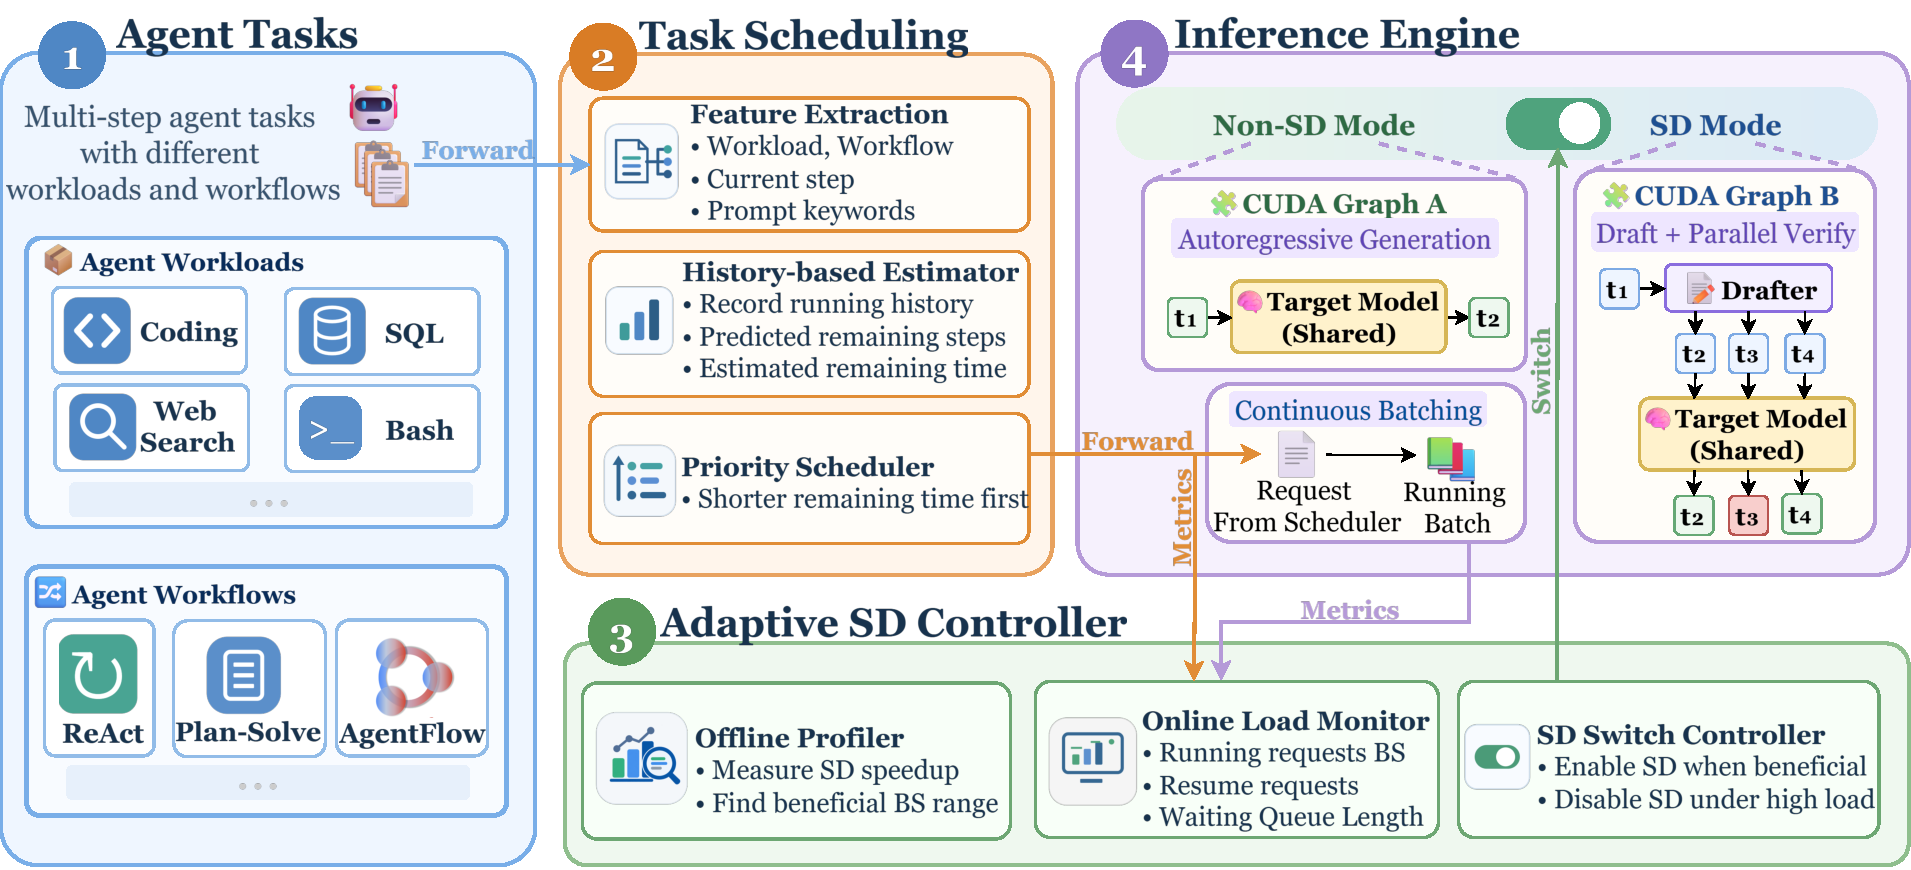
\includegraphics[width=0.9\linewidth]{figures/1-system overview.pdf}
    \end{center}
    \caption{Overview of SpecSys. SpecSys combines remaining-step-aware task scheduling with adaptive SD control. The scheduler estimates the remaining steps of agent jobs and prioritizes shorter jobs, while the SD controller selects between native SD and non-SD execution based on offline profiling and online serving load.}
    \label{fig:overview}
\end{figure}

% 5. 介绍我们的方法(SpecSys)
% 为了解决以上挑战，我们设计了 SpecSyS，引用系统架构图。
To address these challenges, we design SpecSys, an LLM inference system tailored for agent workloads, as shown in \autoref{fig:overview}. 
% SpecSys 在推理引擎的基础上开放了一个可供外部调用的切换开关，能够实现iteration级别的SD与NonSD的模式彻底切换。
Firstly, SpecSys extends the inference engine with an externally controllable switching interface, enabling complete iteration-level switching between native SD and non-SD execution modes.
% 为了降低 agent 任务的端到端时延，SpecSys 在不同的并发度根据不同的性能瓶颈设计了不同的策略。
To reduce the end-to-end latency of agent jobs, SpecSys employs different optimization strategies according to the dominant performance bottleneck under different concurrency.
% 在并发度较低时，SpecSys 会根据离线profile的数据评估 SD 加速比，选择性地调用上述接口启用或禁用 SD，以缓解Decode瓶颈。
Under low concurrency, SpecSys estimates the benefit of SD based on offline profiling results and selectively enables or disables SD through the aforementioned switching interface to alleviate the decoding bottleneck.
% 在并发度较高时，SpecSys 会根据 Agent 任务传入的workload，workflow，当前step，以及prompt中解析得到的关键词，使用历史记录分类查表的方式预测 Agent 任务的剩余 Step 数，然后贪心地选择哪些剩余 Step 数较低的任务，以缓解排队瓶颈。
Under high concurrency, SpecSys uses a lightweight history-based estimator to predict the remaining steps of each agent job based on its workload, workflow, current step, and prompt-derived keywords, and greedily prioritizes jobs with fewer predicted remaining steps to alleviate the queueing bottleneck.

Our contributions can be summarized as follows:
% 5-2. 列举 Contribution
\begin{itemize}
    % 彻底的可供外部调用的 SD-NonSD 切换接口。
    \item \textbf{Externally Controllable SD Switching.}
    We extend the inference engine with an externally controllable switching interface that enables complete iteration-level switching between native SD and non-SD execution modes, reducing runtime overhead by up to 71.3\%.
    % 轻量级的 Agent 任务剩余 Step 预测器。
    \item \textbf{Lightweight Agent Remaining-Step Prediction.}
    We design a lightweight history-based estimator that predicts the remaining steps of an agent job using its workload, workflow, current step, and prompt-derived keywords, achieving an average prediction accuracy of 84.1\% and recall of 82.2\%.
    % 基于并发度联合优化 Agent 任务调度和 SD 切换。
    \item \textbf{Load-Adaptive Agent Scheduling and SD Selection.}
    We selectively enable SD based on offline profiling under low concurrency, while disabling SD and prioritizing jobs with fewer predicted remaining steps under high concurrency.
\end{itemize}

% 6 概括实验
We conduct extensive evaluations of \textsc{SpecSys} across diverse online serving environments, three LLMs, four agent workloads, and three agent workflows. Compared with strong baselines, including ThunderAgent and vLLM with Dynamic SD, \textsc{SpecSys} reduces average job completion time (JCT), achieving from 1.18$\times$  to 2.10$\times$ speedup.

% 2.related work
\section{Related Work}

\subsection{Adaptive Speculative Decoding}
% 背景
% The effectiveness of SD depends on both token acceptance rate and serving load, as low acceptance wastes speculative computation while high serving loads increase batch size and verification cost. 
% To address this, prior work has explored dynamically adjusting the draft length using runtime signals.
% 介绍现有工作
% SpecDec++~\citep{SpecDec++} predicts candidate-token acceptance probabilities and dynamically adjusts the draft length for each drafting round.
% TurboSpec~\citep{TurboSpec} automatically profiles the serving environment and uses a feedback-based controller to dynamically adjust the speculation length at runtime, maximizing LLM serving goodput under varying workloads.
% Nightjar~\citep{Nightjar} similarly adapts the speculative length according to runtime load and batch size to improve the robustness of SD under varying serving conditions.
% vLLM Dynamic SD adjusts the number of speculative tokens according to the current batch size using a configurable batch-size-to-draft-length mapping.
% SGLang Adaptive SD further incorporates token acceptance rate and selects the speculative depth from a configurable batch-size-dependent candidate set.
% 引用更多论文，用简单的话串起来。
Existing token-level adaptive SD approaches can be broadly divided into two categories: one line of work dynamically adjusts drafting parameters, particularly the draft length, based on signals such as token acceptance rate, serving load, batch size, SLOs, and runtime performance~\citep{SpecDec++,TurboSpec,BanditSpec,AdaSpec,Nightjar,Learning_To_Draft}, with similar mechanisms also adopted by vLLM's Dynamic SD~\citep{vLLM} and SGLang's Adaptive SD~\citep{SGLang}.
Another line of work instead focuses on verification optimization, dynamically allocating or pruning the verification workload across requests according to SLOs, token acceptance rate, and system load to improve batched verification efficiency~\citep{AdaServe,D-Cut,ECHO,DSpark}.
% 说明我们与他们的不同
% These approaches primarily focus on adapting the draft length within SD, whereas \sysname determines whether SD should be enabled, making the two directions complementary. 
% Although some existing methods allow the draft length to be reduced to zero, this pseudo-non-SD mode may still retain SD overhead (detailed in~\autoref{dynamic-sd-comparison}). 
% In contrast, \sysname switches directly between native SD and non-SD execution paths, substantially reducing the overhead when SD is disabled. 
% Moreover, existing adaptation policies are typically predefined at engine startup, while \sysname exposes an external runtime interface that allows arbitrary upper-layer policies to control SD dynamically.
% 描述改成更加简便
These approaches optimize SD internally, typically using a zero draft length as a pseudo-non-SD configuration with residual overhead and fixed adaptation logic. 
In contrast, \sysname decides whether to enable SD, switches directly between native SD and non-SD paths, and exposes a runtime interface for arbitrary upper-layer control.


% 介绍 agent 与 SD 结合的论文，说明我们跟他们的区别。
Beyond conventional token-level SD, recent work extends speculation to semantic-level reasoning~\citep{SpecReason,DREAM-R}, and further to agent planning, action, or tool execution~\citep{Interactive_Speculative_Planning,Dynamic_Speculative_Agent_Planning,Speculative_Actions}.
These approaches redesign the upper-level agent workflow, whereas \sysname preserves the workflow and applies SD to LLM inference iterations within each agent task, making the two directions complementary. 
% 简单阐述我们的方法理论上可以拓展到目前新兴的 speculative agent workflows
In principle, our remaining-step prediction method could also be extended to such emerging speculative agent workflows by scaling the predicted number of remaining steps according to the speculative acceptance rate.


\subsection{LLM and Agent Scheduling}


% % 介绍现有工作 - LLM 层面的预测和调度
% Existing LLM serving systems have explored size-based scheduling to mitigate head-of-line blocking and reduce request completion time. 
% SSJF~\citep{SSJF} uses a lightweight proxy model to predict output sequence lengths and prioritizes requests with shorter predicted generations. 
% Learning-to-Rank scheduling~\citep{LTR} instead predicts the relative ordering of output lengths to approximate shortest-job-first (SJF) scheduling without requiring exact length prediction. 
% TRAIL~\citep{TRAIL} further estimates the remaining generation length from intermediate LLM embeddings during decoding and applies a limited-preemption variant of shortest-remaining-processing-time (SRPT) scheduling.

% % 介绍现有工作 - Agent 层面的预测和调度
% Recent agent serving systems further exploit program-level and workflow-level information for scheduling. 
% Autellix~\citep{Autellix} treats agent programs as first-class scheduling units and prioritizes LLM calls based on program-level execution progress. Astraea~\citep{Astraea} incorporates historical execution states and future predictions into a hierarchical scheduler to optimize end-to-end job completion time. ThunderAgent~\citep{ThunderAgent} introduces program-aware scheduling that jointly considers LLM execution, KV-cache states, and tool resources.

% % 说明我们与他们的不同
% % 与 LLM 层面的预测和调度的不同
% Among the above works, some \xiaoxi{please cite} propose scheduling methods based on the estimated remaining generation length of individual \xiaoxirev{steps of} LLM \xiaoxirev{calls within each agent task\footnote{In this work, we use `agent task' and `agent request' interchangeably.}} %requests, 
% \sysname operates at a granularity of the agent task by estimating the remaining steps of an entire agent task across multiple LLM calls \xiaoxi{why task level? as optimizing independently for individual steps might not be the global optimum in reducing the total JCT in the system.}.
% % 与 Agent 层面的预测和调度的不同
% Other agent schedulers \xiaoxi{cite} mainly rely on observed execution states or predictions of near-term execution stages, rather than explicitly estimating the remaining work of the entire agent task. \sysname instead estimates the remaining number of agent steps and uses it to prioritize tasks closer to completion, \xiaoxirev{which follows the shortest-remaining-time-first principle to better approach the global optimum in JCT minimization.}

Existing LLM schedulers optimize individual requests through predicted output lengths or relative length rankings~\citep{SSJF,LTR}, online remaining length estimation~\citep{TRAIL}, preemptive queue-based scheduling~\citep{FastServe}, or %memory-aware and SLO-aware scheduling based on 
estimated future resource demands~\citep{Past-Future,JITServe}. These methods operate primarily at the granularity of individual LLM calls. In contrast, \sysname estimates the remaining steps of an entire agent task\footnote{In this work, we use `agent task' and `agent request' interchangeably.} across multiple LLM calls, since independently prioritizing individual calls may not align with minimizing the end-to-end JCT of agent tasks.

Existing agent schedulers exploit application dependencies and dataflows~\citep{Parrot}, completed-call history or attained service~\citep{Agentix}, historical states and predicted future stages~\citep{Astraea}, program-level execution and resource states~\citep{ThunderAgent}, or workflow structure and cache information~\citep{Helium}. However, they do not explicitly estimate the remaining work of an entire agent task. \sysname instead estimates the remaining number of agent steps and prioritizes tasks closer to completion, following the shortest-remaining-time-first principle at the agent-task level to better align scheduling decisions with end-to-end JCT minimization.



% 3. preliminary
\section{preliminary}

% 介绍推理引擎的执行模式
\subsection{Inference System Execution Modes}
\label{sec:3.1}
% 介绍推理引擎的普通范式
Modern LLM inference systems execute requests iteratively with continuous batching. At each iteration, the \textbf{scheduler} updates the set of running requests and constructs the execution configuration for the current batch. 
The resulting scheduling information is then dispatched to \textbf{workers}, which perform model execution \textbf{\texttt{Execute\_Model}} followed by token processing \textbf{\texttt{Sample\_Tokens}}. 
We therefore abstract each inference iteration as:
\[
\text{Scheduler}
\rightarrow
\text{Workers}\left(
\texttt{Execute\_Model}
\rightarrow
\texttt{Sample\_Tokens}
\right).
\]
% 介绍 Non-SD 和 SD 两种模式的区别
\begin{itemize}
    % Non-SD
    \item \textbf{Non-SD execution mode}. \texttt{Execute\_Model} performs a standard LLM forward pass using a \textbf{decode kernel} and produces logits for the next token of each request.
    \texttt{Sample\_Tokens} then samples the next token from the resulting logits.
    % SD
    \item \textbf{SD execution mode}. \texttt{Execute\_Model} performs LLM verification over multiple draft tokens in parallel using a \textbf{prefill-style kernel} for multi-token queries. \texttt{Sample\_Tokens} then invokes the drafter to generate draft tokens for subsequent verification.
\end{itemize}
% 说明将二者强行统一成一条路径的问题
Consequently, Non-SD and SD differ in both execution flow and kernel usage. Unifying them into a single execution path would require extra alignment or force one mode to use a suboptimal kernel, introducing unnecessary overhead.

% Agent 任务的调度优化问题定义
\subsection{Scheduling Objective for Agent Tasks}

% 简要介绍 agent task 的特点
Unlike conventional LLM tasks, agent tasks are typically executed as multi-step workflows consisting of multiple dependent steps. 
For all serial agent workflows considered in this work, we abstract their execution as a ReAct-style pattern, where LLM inference and tool execution alternate throughout the workflow~\citep{ReAct}. 
As a result, the end-to-end performance of an agent task depends on the execution of the entire workflow rather than the latency of any individual LLM request.

% 每个 agent 请求 R_i 包括 K_i 个 Step，每个 Step 包括一次 LLM 执行和一次 Tool 执行。
For an agent request $R_i$, we represent its workflow as an ordered
sequence of dependent steps,
\begin{equation}
R_i = \langle S_i^1, S_i^2, \ldots, S_i^{K_i} \rangle,
\end{equation}
where $K_i$ denotes the total number of steps of $R_i$.
Each step $S_i^{k}$ consists of an LLM execution followed by an optional tool
execution before the next step can be issued.

% 一个 agent 请求 R_i 在某种调度策略下的总端到端 JCT 的构成
Let $T_{\pi}^{\mathrm{Queue}}(S_i^j)$ denote the waiting time of step $S_i^j$ under scheduling policy $\pi$, $T^{\mathrm{LLM}}(S_i^j)$ denote its LLM execution time, and $T^{\mathrm{Tool}}(S_i^j)$ denote the tool execution time. The end-to-end Job Completion Time (JCT) of the agent request $R_i$ can be expressed as
\begin{equation}
\mathrm{JCT}_{\pi}(R_i) = \sum_{j=1}^{K_i} \left( T_{\pi}^{\mathrm{Queue}}(S_i^j) + T^{\mathrm{LLM}}(S_i^j) \right) + \sum_{j=1}^{K_i-1} T^{\mathrm{Tool}}(S_i^j).
\end{equation}

% 优化问题：最小化一组 Agent 任务的平均端到端 JCT
Given a set of agent requests $\mathcal{R}$, our scheduling objective is to find a feasible scheduling policy $\pi$ that minimizes the average end-to-end JCT:
\begin{equation}
\pi^{*} = \arg\min_{\pi \in \Pi} \frac{1}{|\mathcal{R}|} \sum_{R_i \in \mathcal{R}} \mathrm{JCT}_{\pi}(R_i),
\end{equation}
where $\Pi$ denotes the set of feasible scheduling policies that respect the dependency between agent steps and the serving capacity of the inference system.

% 引用论文说明这个优化问题是 NP-Hard
This global scheduling objective is computationally challenging due to the dependencies among agent steps and the contention among concurrent requests. 
Astraea~\citep{Astraea} formalizes a similar multi-stage agent scheduling problem and has proved it to be NP-hard. 
Therefore, practical online agent serving systems typically rely on efficient   euristic policies to approximate the optimal schedule.

% 4. method
\section{Method}
% SD 状态切换示意图
\begin{figure}[t]
    \vspace{-20pt}
    \begin{center}
    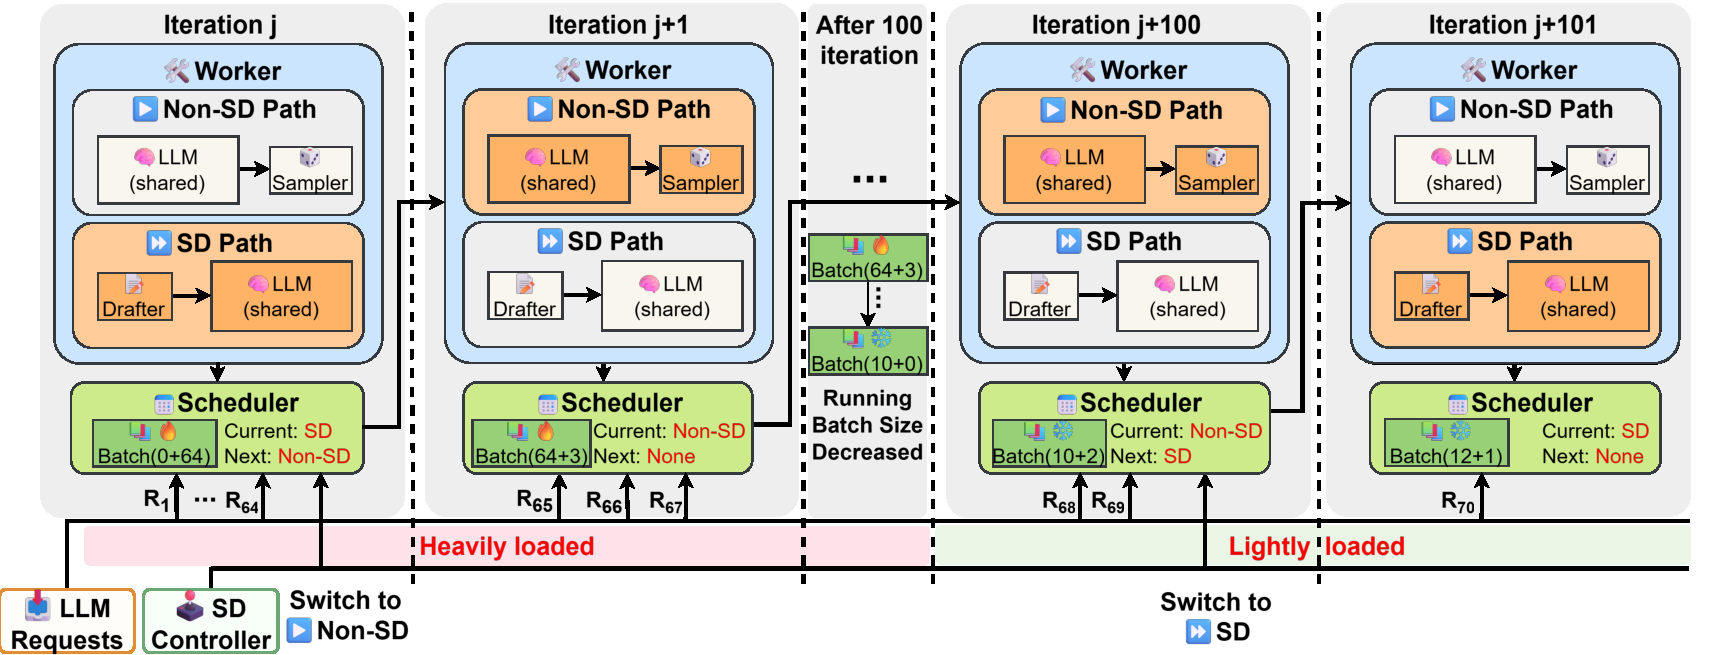
\includegraphics[width=1.0\linewidth]{figures/method-overview.pdf}
    \end{center}
    \vspace{-10pt}
    % \caption{
    %     Illustration of iteration-level SD switching in \sysname.
    %     At iteration $i$, a heavily loaded batch triggers a \emph{Switch to Non-SD} request, which is forwarded by the scheduler and takes effect at iteration $i+1$.
    %     Similarly, a \emph{Switch to SD} request issued under light load at iteration $i+2$ takes effect at iteration $i+3$.
    %     All requests within an iteration follow the same execution mode.
    % }
    \caption{
    Illustration of iteration-level SD switching in \sysname.
    At iteration $j$, 64 incoming requests drive the system into a heavily loaded state, causing the external SD Controller to issue a switch-to-Non-SD request.
    The internal Scheduler applies the request at iteration $j+1$, and inference proceeds along the native Non-SD path for the next 100 iterations as the running batch size gradually decreases.
    After the system becomes lightly loaded, the SD Controller issues a switch-to-SD request, which takes effect at iteration $j+101$, after which inference continues along the native SD path.
    }
    \label{fig:sd_switch}
\end{figure}

% 1.支持 SD 动态切换的外部接口
\subsection{Externally Controllable SD Switching}
\label{sec:4.1}
% 总起，分成三部分：外部接口，scheduler，worker
% To support customizable SD selection policies at the upper layer, \sysname extends the underlying inference engine with an externally controllable runtime SD switch  \xiaoxi{emphasize the existing dynamic SD pre-sets a static switching condition, and more importantly, their default path is fixed to the SD Path, resulting a xxxx overhead.}.


Existing dynamic SD approaches have two limitations. First, their switching logic is embedded within the inference engine, limiting customized upper-layer control. Second, disabling SD does not necessarily restore the native non-SD path: %their non-SD mode is still confined to the SD path, %retaining substantial residual overhead. 
% as shown in~\autoref{tab:token_consistency_form} and~\autoref{fig:nonsd_overhead_b32}.
as shown in~\autoref{tab:token_consistency_form}, vLLM Dynamic SD (vLLM-DSD) and SGLang Adaptive SD (SGLang-ASD) with zero draft length remain token-consistent with native SD but not with native Non-SD, indicating that they still follow the SD path 
(detailed in~\autoref{dynamic-sd-comparison}). %The resulting overhead is shown in~\autoref{fig:nonsd_overhead_b32}.
\sysname %exposes an externally controllable runtime interface that 
addresses these issues by decoupling mode selection logic from engine execution and switching directly between native SD and non-SD paths, significantly reducing non-SD overhead (see~\autoref{fig:nonsd_overhead_b32}). As shown in~\autoref{fig:sd_switch}, this design consists of three components: %an external control interface, an iteration-level state transition in the scheduler, and path-specific execution paths in the worker (Figure~\autoref{fig:sd_switch}).
% \xiaoxi{Please change the description of Figure~\ref{fig:sd_switch} to the phenomenon/benefit of switching.} 

% \xiaoxi{Move Table~\ref{tab:token_consistency} and Figure~\ref{fig:nonsd_overhead} here in a compact way.}


% 描述 existing dynamic SD 方法的问题：没有彻底切换，存在overhead
\begin{figure}[b]
    \vspace{-10pt}
    \centering
    % =========================
    % Left: Table
    % =========================
    \begin{minipage}[t]{0.73\linewidth}
        \centering
        \captionof{table}{Token consistency across adaptive SD approaches.}
        \label{tab:token_consistency_form}
    
        \resizebox{\linewidth}{!}{
        \begin{tabular}{cccc}
            \toprule
            \textbf{Inference Engine} &
            \textbf{Approach} &
            \textbf{Non-SD} &
            \textbf{SD} \\
            \midrule
    
            \multirow{3}{*}{vLLM}
            & Dynamic SD ($\text{draft\_len}=0$)
            & $\times$ & $\checkmark$ \\
    
            & SpecSys-NonSD
            & $\checkmark$ & -- \\
    
            & SpecSys-SD
            & -- & $\checkmark$ \\
    
            \midrule
    
            \multirow{3}{*}{SGLang}
            & Adaptive SD ($\text{draft\_len}=0$)
            & $\times$ & $\checkmark$ \\
    
            & SpecSys-NonSD
            & $\checkmark$ & -- \\
    
            & SpecSys-SD
            & -- & $\checkmark$ \\
    
            \bottomrule
        \end{tabular}
        }
    \end{minipage}
    \hfill
    % =========================
    % Right: Figure
    % =========================
    \begin{minipage}[t]{0.26\linewidth}
        \vspace{0pt}
        \centering
        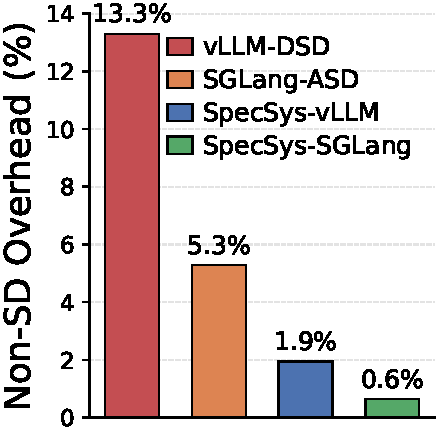
\includegraphics[width=\linewidth]{figures/nonsd_overhead_bs32.pdf}
        \setlength{\abovecaptionskip}{-15pt}
        \captionof{figure}{Non-SD Path Overhead of Adaptive SD}
        \label{fig:nonsd_overhead_b32}
    \end{minipage}

\end{figure}


% 外部接口
\textbf{External Control Interface.}
% \sysname extends the inference engine with a lightweight control interface to receive SD switching requests and forward them to the scheduler to update the desired execution mode.
% This design decouples the external scheduling policy from the internal execution logic of the inference engine. \xiaoxi{still need to highlight the fundamental benefit, e.g., improved deployment flexibility or extendibility}
\sysname exposes a lightweight control interface that receives SD switching requests and forwards them to the scheduler to update the desired execution mode.
This design decouples the switching policy from internal execution logic, allowing customized policies to be changed or replaced without modifying the underlying inference engine.
%As a result, \sysname can be flexibly integrated with different deployment environments and external scheduling strategies.

% scheduler
\textbf{Iteration-Level State Transition.}
% To ensure execution consistency, \sysname performs SD switching only at inference-iteration boundaries \xiaoxi{A better way to highlight our method that enables iteration-level switching should be relating this iteration-level switching to the purpose of reducing JCT in addition to execution consistency}. 
%To eliminate the lag between external control and internal execution introduced by this decoupled design, \sysname adopts iteration-level switching, allowing switching requests to take effect at the next inference iteration.
%Specifically, the scheduler maintains a current mode and an expected mode. External requests update only the expected mode, which is applied to the worker at the next iteration boundary.
Serving conditions can change while a continuous batch remains active, so coarse-grained reconfiguration may delay a needed switch. \sysname therefore applies mode changes at inference-iteration boundaries, so controller decisions take effect at the next iteration without disrupting the current one. The scheduler tracks current and next modes; external requests update the next mode, which is then propagated to the worker.

% worker
\textbf{Path-Specific Worker Execution.}
% As Non-SD and SD follow different execution paths (in~\autoref{sec:3.1}), \sysname preserves separate execution branches for the two paths. 
% During engine initialization, CUDA Graphs for both modes are prepared in advance. \xiaoxi{Should point out the importance or challenging issue related to CUDA graphs in the switching.}
% At runtime, the worker selects the corresponding execution branch and CUDA Graph based on the mode specified in \texttt{SchedulerOutput}. 
% Within each iteration, all requests in the batch follow the same execution mode and therefore share the same execution path, ensuring consistent batch execution while enabling low-overhead iteration-level switching.
Existing dynamic SD approaches focus on the SD path and provide limited optimization for native Non-SD execution, especially dedicated CUDA Graphs. Extending switching to two native paths therefore requires optimizing both paths independently. 
\sysname prepares CUDA Graphs for both paths during initialization, and the worker uses the pre-captured CUDA Graph corresponding to the selected path in each iteration.



% 2.Agent 剩余 step 数预测
\subsection{Agent Remaining-Step Prediction}
\label{sec:4.2}
% 介绍预测方法的动机
% \xiaoxirev{To realize an efficient scheduling mechanism that exploits unique characteristics of agent workloads, we conduct a profiling experiment
% %Based on our profiling results 
% (\autoref{step-distribution}), which reveals two insights}: {\em (i) Agent execution patterns vary across workflows and workloads. (ii) The prompts of LLM inference steps provide useful information of the current execution state that can guide scheduling decisions}. 
% First, we categorize today's agent workflows into three types:

% \xiaoxi{cite references below, for the workflow terminologies that appear in the first time}
% \begin{itemize}[leftmargin=10pt]
%     \item \textbf{Type A} represents planning-based workflows, such as Plan-and-Solve, where the planned step count can be directly extracted from the prompt, making prediction straightforward.
%     \item \textbf{Type B} represents multi-step iterative workflows, such as AgentFlow, where tasks terminate at specific step boundaries and exhibit a multimodal step distribution, making the completion step easier to estimate using the mode of the historical distribution.
%     \item \textbf{Type C} represents step-by-step workflows, such as ReAct, where tasks may terminate at almost any step, making prediction more difficult and requiring additional execution-state information.
% \end{itemize}
To exploit agent-specific execution patterns for remaining-step prediction, we profile representative agent workflows and categorize them into three types:
%To realize an efficient scheduling mechanism that exploits unique characteristics of agent workloads, we conduct a profiling experiment
%Based on our profiling results 
%(\autoref{step-distribution}), which reveals two insights: {\em (i) Agent execution patterns vary across workflows and workloads. (ii) The prompts of LLM inference steps provide useful information of the current execution state that can guide scheduling decisions}. 
%First, we categorize today's agent workflows into three types:

% \begin{itemize}[leftmargin=10pt]\label{type-describe}
%     \item \textbf{Type A} represents planning-based workflows, such as Plan-and-Solve, where the planned step count can be directly extracted from the \xiaoxirev{planning output}, making prediction straightforward.
%     \item \textbf{Type B} represents multi-step iterative workflows, such as AgentFlow, where tasks terminate at specific step boundaries and exhibit a multimodal step distribution, making the completion step easier to estimate using the mode of the historical distribution.
%     \item \textbf{Type C} represents step-by-step workflows, such as ReAct, where tasks may terminate at almost any step, making prediction more difficult and requiring additional execution-state information.
% \end{itemize}

\begin{itemize}[leftmargin=10pt]\label{type-describe}
    \item \textbf{Type A} represents planning-based workflows, such as Plan-and-Solve, where the planned step count can be extracted from the planning output. %, making prediction straightforward. 
    A parsing example is provided in~\autoref{prompt_parser}.
    \item \textbf{Type B} represents multi-step iterative workflows, such as AgentFlow, where tasks terminate at specific step boundaries and exhibit a multimodal step distribution (see~\autoref{step-distribution}), enabling completion-step  estimation from historical distributions.
    \item \textbf{Type C} represents step-by-step workflows, such as ReAct, where tasks may terminate at almost any step, requiring additional execution-state information for prediction.
\end{itemize}
Across these workflow types, our profiling identifies two complementary signals for remaining-step prediction: historical execution patterns conditioned on workflow and workload, and execution-state cues exposed by the current LLM-call prompt.

% 解析请求附带的信息，提取状态关键词，然后分类。
\textbf{Request-Level Information Extraction.}
For each LLM request, the upstream agent application provides its workflow, workload, and current execution step as metadata. 
\sysname further parses the prompt for keywords indicating {\em errors, repeated actions, completion, and termination}, and maps the request to a workflow-specific {\em execution state}.
Concrete examples are provided in~\autoref{prompt_parser}.

% 分类保存历史记录
\textbf{Offline History Profiling.}
% \sysname groups completed agent requests by workflow and workload and records the distribution of total execution steps $T$. 
% The distributions are further conditioned on the extracted execution state and, for Type C workflows, the transition between the previous and current states. \xiaoxi{mention the profiling cost is not large.}
\sysname groups completed agent requests by workflow and workload and records the distribution of total execution steps $T$. 
The distributions are further conditioned on the extracted execution state and, for Type C workflows, the transition between the previous and current states.
The profiling cost is negligible, as \sysname only maintains lightweight statistics over completed requests and performs no additional computation on the online serving path.

% \xiaoxi{Please explain the reason/intuition of each specific way/parameter used in the following estimation for different workflow types. Make them tightly related to your observations.}

% 剩余 step 数估计
\textbf{Remaining-Step Estimation.}
% todo: 解释一下为什么要用这样的方法
%\sysname adopts different estimation strategies based on the characteristics of each workflow type as described in~\autoref{type-describe}.
For each workflow type, \sysname estimates the remaining steps using workflow-specific signals. Let $\hat{R}_x$ denote the estimate for Type $x$. Type A leverages the explicit plan; Type B uses the most frequent historical completion step to capture recurring termination patterns; Type C further incorporates state transitions and uses the median for more robust estimation.

% Type A，解析 plan 直接得到 P ，然后 P-k 得到剩余 step
For \textbf{Type A}, let $P$ denote the planned step count extracted from the prompt. 
Given the current step $k$, the remaining steps are directly computed as
\begin{equation}
\hat{R}_{A} = \max(0, P-k).
\end{equation}

% Type B，看当前状态，根据对应的分类槽里的历史信息中的条件众数得到预测结果
For \textbf{Type B}, let $s_k$ denote the execution state at step $k$. 
\sysname estimates the completion step using the mode of the historical distribution conditioned on the current step and execution state:
\begin{equation}
\hat{T}_{B} =
\mathrm{mode}\{T \mid k, s_k\},
\qquad
\hat{R}_{B} = \max(0, \hat{T}_{B}-k).
\end{equation}

% Type C，看当前状态+历史状态，根据对应的分类槽里的历史信息中的条件中位数得到预测结果
For \textbf{Type C}, \sysname further conditions the historical records on both the previous state $s_{k-1}$ and current execution state $s_k$ and uses the median of the corresponding historical distribution:

\begin{equation}
\hat{T}_{C} =
\mathrm{median}\{T \mid k, s_{k-1}, s_k\},
\qquad
\hat{R}_{C} = \max(0, \hat{T}_{C}-k).
\end{equation}

When the fine-grained statistics are insufficient, \sysname progressively falls back to the current-state-conditioned distribution and then to the workflow-workload-level historical distribution.


% 3.基于动态负载的 Agent 任务调度和 SD 选择
\subsection{Load-Adaptive Agent Scheduling and SD Selection}
\label{sec:4.3}

% 离线 profile 出不同配置下的 SD加速比与推理负载的关系，得到一个平衡点。
\textbf{Offline SD Speedup Profiling.}
\label{sec:4.3.1}
For each model and hardware configuration, \sysname profiles SD speedup across different batch sizes before engine startup and identifies the break-even load $B^{*}$, defined as the largest batch size at which SD achieves a speedup greater than or equal to 1. 
SD is beneficial below $B^{*}$, while its overhead can cause performance degradation above this point. Detailed profiling results are provided in~\autoref{sd-speedup}.

% 负载估计
\textbf{Future-Load Estimation.}
% 因为切换存在一定的滞后性。考虑负载时不仅是看推理引擎内部的running batch size，还要看外部proxy的计划resume的任务数，二者相加得到预测的未来负载。
Since SD switching takes effect with a short delay, the current running batch size alone may not reflect the load when the new mode becomes active. 
\sysname therefore also considers agent requests temporarily held by the router-proxy that are scheduled to be resumed and submitted to the inference engine. 
Specifically, it estimates the near-future load by combining the current running batch size $B_{\mathrm{running}}$ with the number of requests to be resumed $B_{\mathrm{resume}}$:
\begin{equation}
\hat{B}=B_{\mathrm{running}}+B_{\mathrm{resume}}.
\end{equation}

% 基于负载选择性使用SD
\textbf{Load-Adaptive SD Selection.}
\sysname compares the estimated load $\hat{B}$ with the profiled break-even load $B^{*}$ and sends an SD-switching request to the inference engine interface accordingly. The SD execution mode is determined as
\begin{equation}
\mathrm{Enable\mbox{-}SD} =
\begin{cases}
\mathrm{True},  & \hat{B} \leq B^{*}, \\
\mathrm{False}, & \hat{B} > B^{*}.
\end{cases}
\end{equation}
This strategy enables SD under low load to mitigate the decode bottleneck.

% 高负载下的任务调度策略
\textbf{Agent Task Scheduling.}
When the serving load becomes high and agent tasks start queuing at the router-proxy, \sysname prioritizes the task with the fewest predicted remaining steps:
\begin{equation}
j^{*} =
\operatorname*{arg\,min}_{j \in \mathcal{Q}}
\hat{R}_{j},
\end{equation}
where $\mathcal{Q}$ denotes the queued agent tasks and $\hat{R}_{j}$ is the remaining steps of task $j$ estimated by the predictor in~\autoref{sec:4.2}.
This strategy prioritizes tasks closer to completion, thereby mitigating the queue bottleneck under high serving load.

% 5. experiments
\section{experiments}

\subsection{setups}
Environment: 4090, A100

Model: Qwen3-14B, Qwen3-32B, ... 
Workload \& Datasets: Coding(MBPP), Web Search(2Wiki), Bash(NL2Bash), SQL(Spider)
Agent Workflow: ReAct, Plan-And-Slove, AgentFlow
Inference Trace: Azure, Qwen-Bailian

% 6. conclusion
% 总结
\section{conclusion}
In this work, we present SpecSys, an efficient inference system that jointly optimizes speculative decoding and task scheduling for LLM-powered agents under dynamic serving loads.
By exposing a low-overhead runtime interface that enables complete iteration-level switching between native SD and Non-SD execution, selectively enabling SD under low serving loads, and prioritizing tasks with fewer predicted remaining steps under high serving loads, SpecSys adapts to the changing performance bottlenecks of online agent serving to minimize average job completion time (JCT).
Extensive evaluations across three LLMs, two hardware platforms, four agent workloads, three agent workflows, and two real-world online serving traces show that SpecSys consistently improves end-to-end performance, achieving 1.18$\times$--2.10$\times$ speedups over the best baselines.

\clearpage

% 7. statement
\subsection*{AI Use Statement}

In this work, we used generative AI tools to assist with writing, information retrieval and discovery, and research ideation and execution.

For writing, generative AI was used to assist with drafting, polishing, and checking the formatting of the manuscript. For retrieval and discovery, generative AI was used to summarize literature and identify related work and relevant sources. For research ideation and execution, generative AI was used to assist with code understanding, simple script generation, code review, debugging, and identifying potential technical issues.

All AI-assisted outputs were reviewed by the authors. Suggested literature and references were checked against the original sources, AI-assisted code and debugging suggestions were manually inspected and validated through execution and testing, and AI-assisted manuscript text was reviewed and revised for technical correctness and consistency with the reported results.

We take responsibility for the final content of this work, including all text, claims, code, and other artifacts produced with the aid of generative AI.

% \subsection*{Ethics statement}

% (This section is \textbf{recommended} and does not count toward the page limit.)

% If authors feel that their paper submission raises questions regarding the Code
% of Ethics, they are encouraged to include a paragraph of Ethics Statement (at
% the end of the main text before references) to address potential concerns where
% appropriate. Topics include, but are not limited to, studies that involve human
% subjects, practices to data set releases, potentially harmful insights,
% methodologies and applications, potential conflicts of interest and sponsorship,
% discrimination/bias/fairness concerns, privacy and security issues, legal
% compliance, and research integrity issues (e.g., IRB, documentation, research
% ethics). This statement should not be more than 1 page.


\section*{Reproducibility Statement}

We make extensive efforts to facilitate the reproducibility of SpecSys.  Additional details required to reproduce our experiments are provided in the appendix. In particular, \autoref{app:hyperparameters} reports the agent-trace collection and replay procedure, inference-engine and generation configurations, speculative decoding settings, scheduling parameters, and software environments. \autoref{prompt_parser} provides concrete examples and implementation details of the feature extraction and remaining-step prediction procedures for different workflow types. We further report the workload and request characteristics, hardware serving capacity, and online trace statistics in~\autoref{request-and-resource-analysis} and~\autoref{online-trace-detail}. The profiling methodology and configuration-dependent thresholds used for selective SD are documented in~\autoref{sd-speedup}. Together, these descriptions specify the workloads, serving environments, system configurations, and implementation choices used throughout our evaluation. We have also released the SpecSys source code and the collected agent execution trajectories in an anonymous public repository at \url{https://anonymous.4open.science/r/SpecSys-Code-E03D/} to facilitate reproduction of our results.





% \subsubsection*{Acknowledgments}
% Use unnumbered third level headings for the acknowledgments. All
% acknowledgments, including those to funding agencies, go at the end of the paper.

% references
\bibliography{iclr2027_conference}
\bibliographystyle{iclr2027_conference}

\clearpage

% 8. appendix
\appendix

% Agent任务的 LLM 时间占比与瓶颈
\section{LLM Time Breakdown and Bottleneck Analysis in Agent Tasks}
\label{llm-time-ratio}

\begin{table}[H]
    \vspace{-10pt}
    \centering
    \caption{LLM inference time breakdown across agent tasks.}
    \label{tab:llm_time_breakdown}
    \begin{tabular}{llccc}
        \toprule
        \textbf{Task} & \textbf{Dataset} & \textbf{Avg. JCT (s)} & \textbf{Avg. LLM Time (s)} & \textbf{LLM Time Ratio} \\
        \midrule
        Web Search & 2WikiMultihopQA & 60.36 & 36.49 & 60.46\% \\
        Web Search & Bamboogle       & 49.15 & 32.91 & 66.95\% \\
        Web Search & HotpotQA        & 40.72 & 29.14 & 71.56\% \\
        Coding     & MBPP            & 30.10 & 30.06 & 99.87\% \\
        \bottomrule
    \end{tabular}
\end{table}

\begin{figure}[!b]
    \begin{center}
    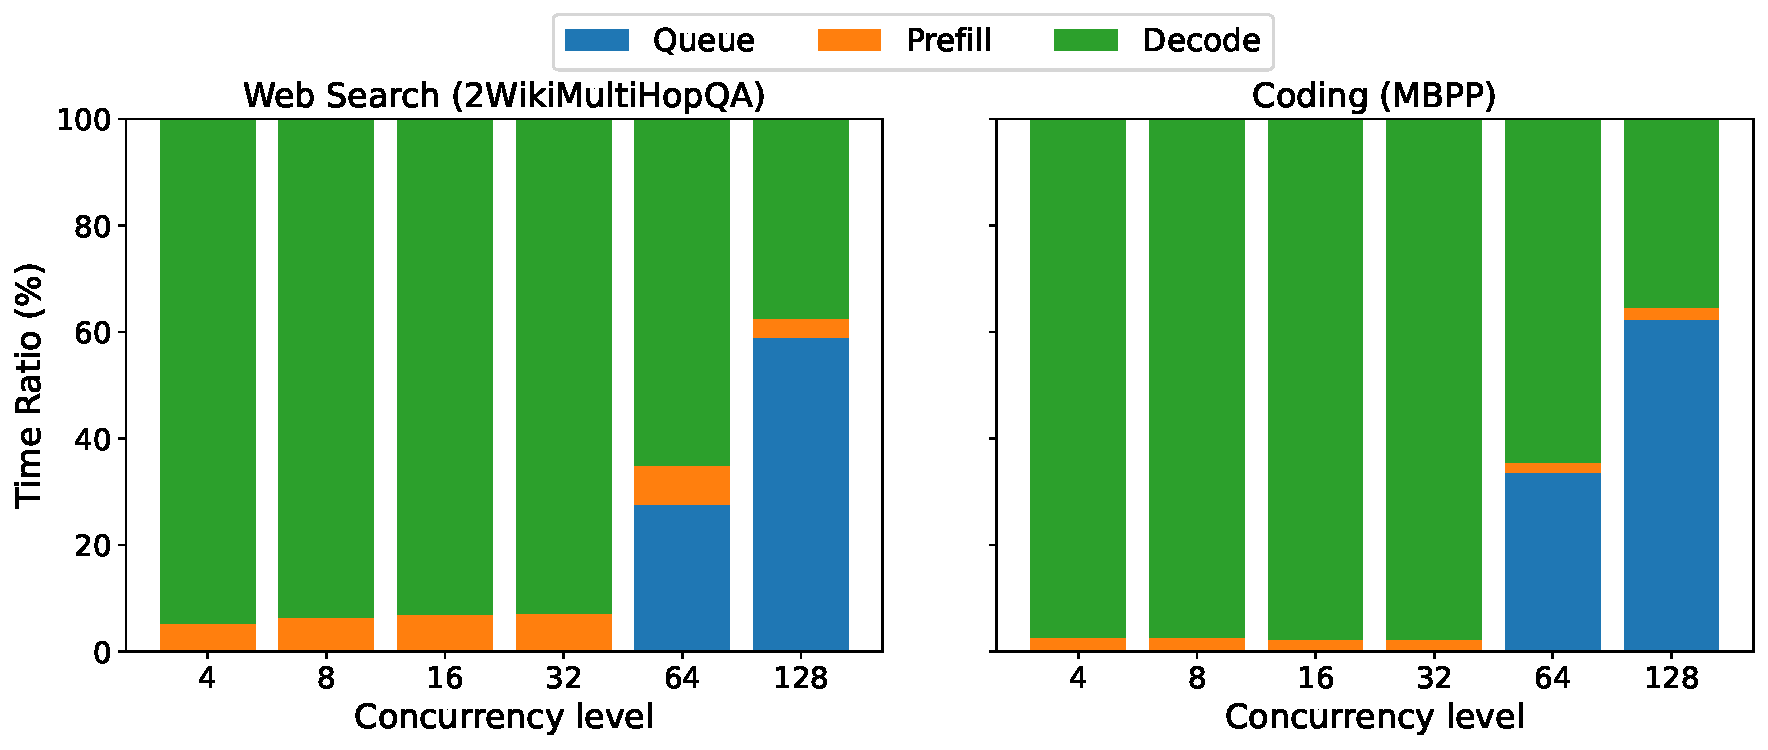
\includegraphics[width=1.0\linewidth]{figures/5-time-ratio.pdf}
    \end{center}
    \caption{
        LLM inference time breakdown under different concurrency levels for two agent tasks, Web Search on 2WikiMultihopQA and Coding on MBPP, showing a shift from decode-dominated latency at low concurrency to queue-dominated latency at high concurrency.
    }
    \label{fig:llm_time_ratio}
\end{figure}

We measure the end-to-end execution time and the fraction spent on LLM inference across different agent tasks and datasets, as shown in~\autoref{tab:llm_time_breakdown}.
LLM inference accounts for the majority of the end-to-end latency across all evaluated settings.
For some tasks, the execution time of external tools is negligible, making LLM inference responsible for nearly all of the overall latency.
These results indicate that the end-to-end latency of agent tasks is primarily bottlenecked by LLM inference.
Coding and Web Search tasks typically represent two contrasting cases.
In Coding tasks, the tool execution mainly consists of running generated code and is usually very fast, whereas in Web Search tasks, the agent often needs to retrieve and access multiple webpages, making tool execution more sensitive to network latency.
Despite this difference, LLM inference still accounts for a substantial fraction of the end-to-end latency in both types of tasks.

We further analyze the latency breakdown of LLM requests in agent tasks, as shown in~\autoref{fig:llm_time_ratio}.
The latency of an LLM request mainly consists of three components: prefill, decode, and queueing time.
Existing serving systems have extensively optimized KV-cache reuse, substantially reducing redundant computation during the prefill stage and making prefill latency relatively small.
To preserve KV-cache residency and avoid excessive eviction or recomputation, these systems typically employ admission control based on the number of concurrent requests and the available KV-cache capacity.
When the number of concurrent requests exceeds the capacity that can be supported by the available KV cache, newly arrived requests are queued and can enter inference only after running requests complete and release their KV-cache space.

Based on these results, we observe a concurrency-dependent shift in the LLM inference bottleneck of agent tasks.
At low concurrency, decode time dominates the request latency and serves as the primary performance bottleneck.
As concurrency increases, more requests are blocked by admission control, causing queueing time to grow rapidly and eventually dominate the overall latency.
As a result, the performance bottleneck shifts from decoding at low serving loads to queueing at high serving loads.

\clearpage

% Agent任务使用 SD 的加速比随 Batch Size 的变化关系
\section{Impact of Batch Size on SD Speedup for Agent Tasks}
\label{sd-speedup}

% 暂时占个位置
\clearpage

% 对比不同动态 SD 方法
\section{Comparison of Dynamic SD Approaches.}
\label{dynamic-sd-comparison}

\begin{table}[H]
    \vspace{-20pt}
    \centering
    \caption{Token consistency comparison across different approaches of dynamic SD.}
    \label{tab:token_consistency}
    \begin{tabular}{cccc}
        \toprule
        \textbf{Inference Engine} & \textbf{Engine A} & \textbf{Engine B} & \textbf{Token Consistency} \\
        \midrule

        \multirow{4}{*}{vLLM}
        & Dynamic SD ($\text{draft\_len}=0$)
        & NonSD
        & $\times$ \\

        & Dynamic SD ($\text{draft\_len}=0$)
        & SD
        & $\checkmark$ \\

        & SpecSys-NonSD Mode
        & NonSD
        & $\checkmark$ \\

        & SpecSys-SD Mode
        & SD
        & $\checkmark$ \\

        \midrule

        \multirow{4}{*}{SGLang}
        & Adaptive SD ($\text{draft\_len}=0$)
        & NonSD
        & $\times$ \\

        & Adaptive SD ($\text{draft\_len}=0$)
        & SD
        & $\checkmark$ \\

        & SpecSys-NonSD Mode
        & NonSD
        & $\checkmark$ \\

        & SpecSys-SD Mode
        & SD
        & $\checkmark$ \\

        \bottomrule
    \end{tabular}
\end{table}

\textbf{Token Consistency across Dynamic SD Approaches.}
Online inference engines typically employ different execution paths for SD and Non-SD generation to improve efficiency, with different kernels used for key computations such as attention.
As a result, even under deterministic decoding settings (i.e., temperature $=0$ and top-$k=1$), SD and Non-SD execution may generate slightly different token sequences for the same prompt due to differences in their underlying computation paths, although the generated contents are usually semantically similar.
Therefore, token-level consistency provides a practical indicator of whether two execution modes follow the same underlying inference path.
We evaluate this behavior for two dynamic SD approaches, vLLM Dynamic SD and SGLang Adaptive SD, as shown in~\autoref{tab:token_consistency}.
For both vLLM Dynamic SD and SGLang Adaptive SD, when SD is disabled by setting $\text{draft\_len}=0$, the generated tokens are inconsistent with those of the native Non-SD engine but remain consistent with those produced by the native SD engine.
This indicates that setting $\text{draft\_len}=0$ does not fully switch execution back to the native Non-SD path; instead, the engine continues to follow the SD execution path with SD disabled.
In contrast, SpecSys's Non-SD mode produces tokens consistent with the native Non-SD engine, while its SD mode remains consistent with the native SD engine.
These results demonstrate that SpecSys performs a more complete runtime switch between the native SD and Non-SD execution paths.

\textbf{Non-SD Overhead across Dynamic SD Approaches.}
Since vLLM Dynamic SD and SGLang Adaptive SD continue to execute along the SD path when $\text{draft\_len}=0$, this path is suboptimal for autoregressive Non-SD generation and introduces additional performance overhead.
We therefore measure the Non-SD execution overhead of these two dynamic SD approaches and SpecSys relative to the native Non-SD engine, as shown in~\autoref{fig:nonsd_overhead}.
However, SpecSys consistently incurs substantially lower overhead than vLLM Dynamic SD and SGLang Adaptive SD across all batch sizes.
These results further demonstrate the benefit of SpecSys's more complete runtime switching between the native SD and Non-SD execution paths.

\begin{figure}[!b]
    \begin{center}
    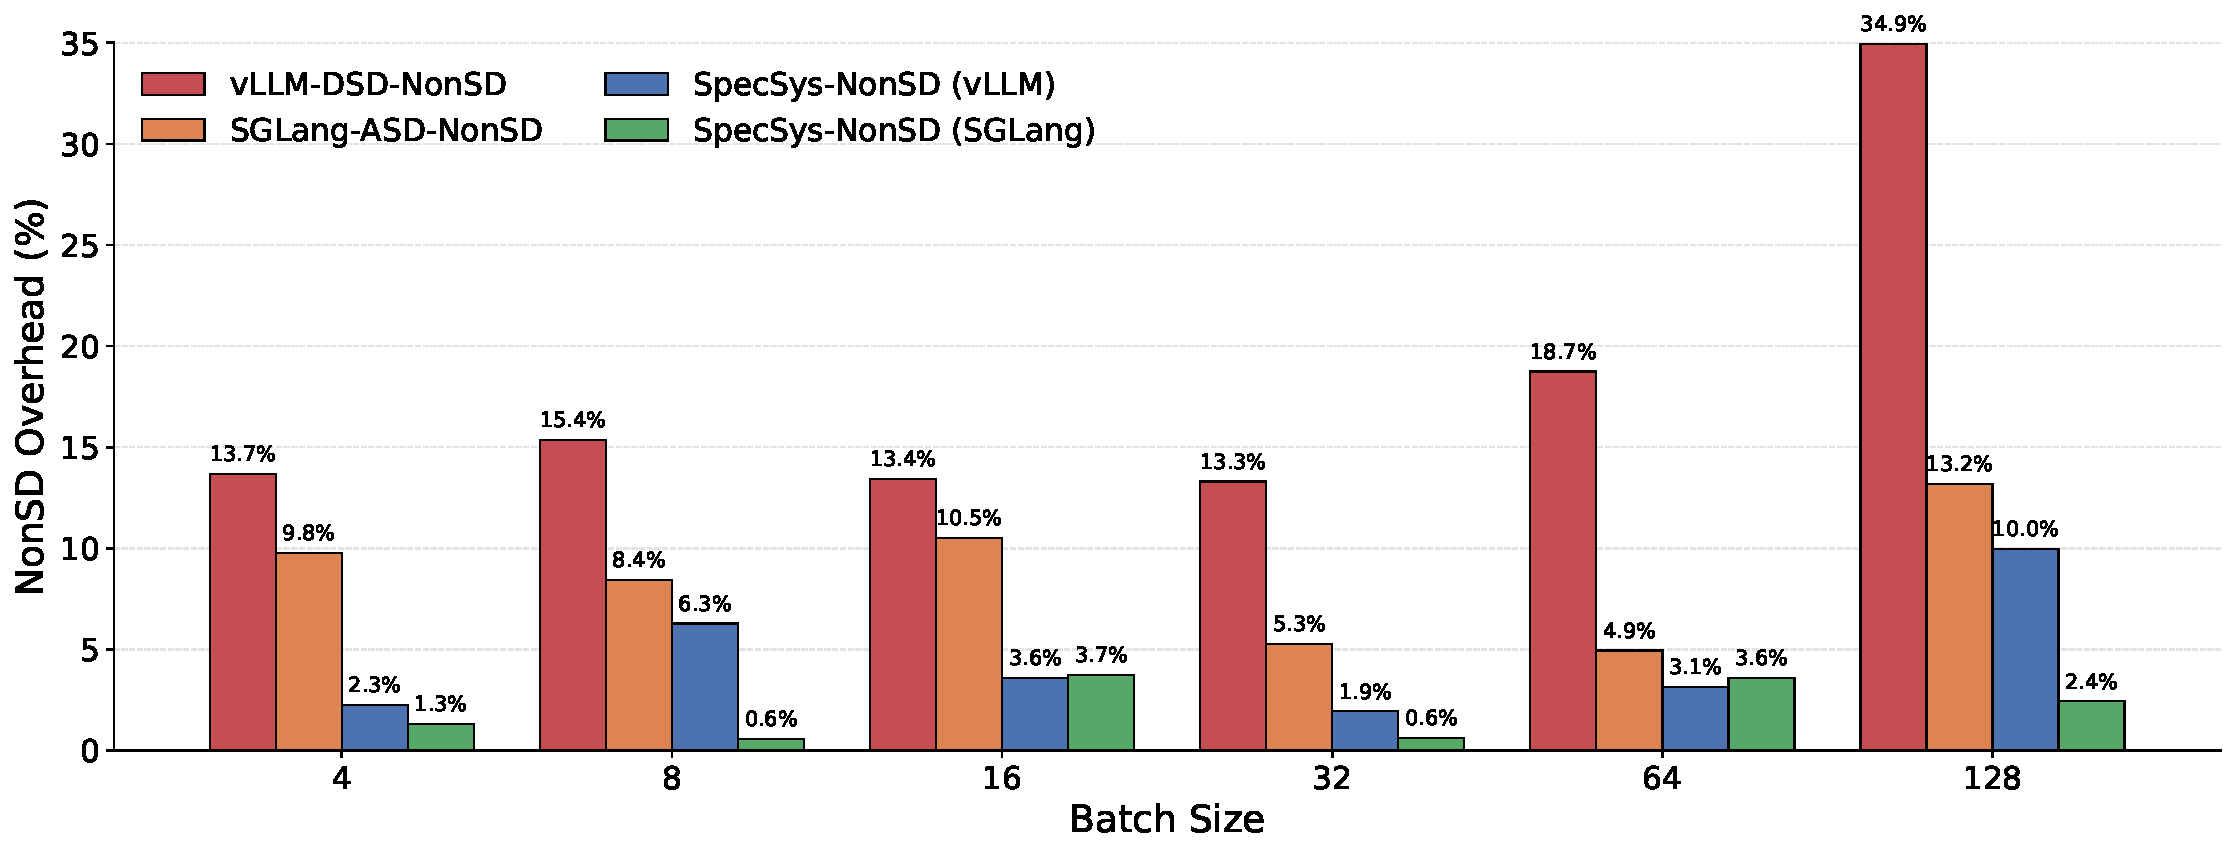
\includegraphics[width=1.0\linewidth]{figures/6-nonsd-overhead.pdf}
    \end{center}
    \caption{
        Non-SD execution overhead across different dynamic SD approaches and batch sizes.
    }
    \label{fig:nonsd_overhead}
\end{figure}


% 列举不同 workflow 和 workload 的 step 分布
\section{Agent Step Distributions across Workflows and Workloads}
\label{step-distribution}

% 暂时占个位置
\clearpage

% prompt 解析的实例
\section{Examples of Prompt Parsing}
\label{prompt_parser}

% 暂时占个位置
\clearpage

% 轨迹的请求变化图
\section{Request Arrival Patterns of Online Serving Traces}
\label{online-trace-detail}

\begin{figure}[H]
    \begin{center}
    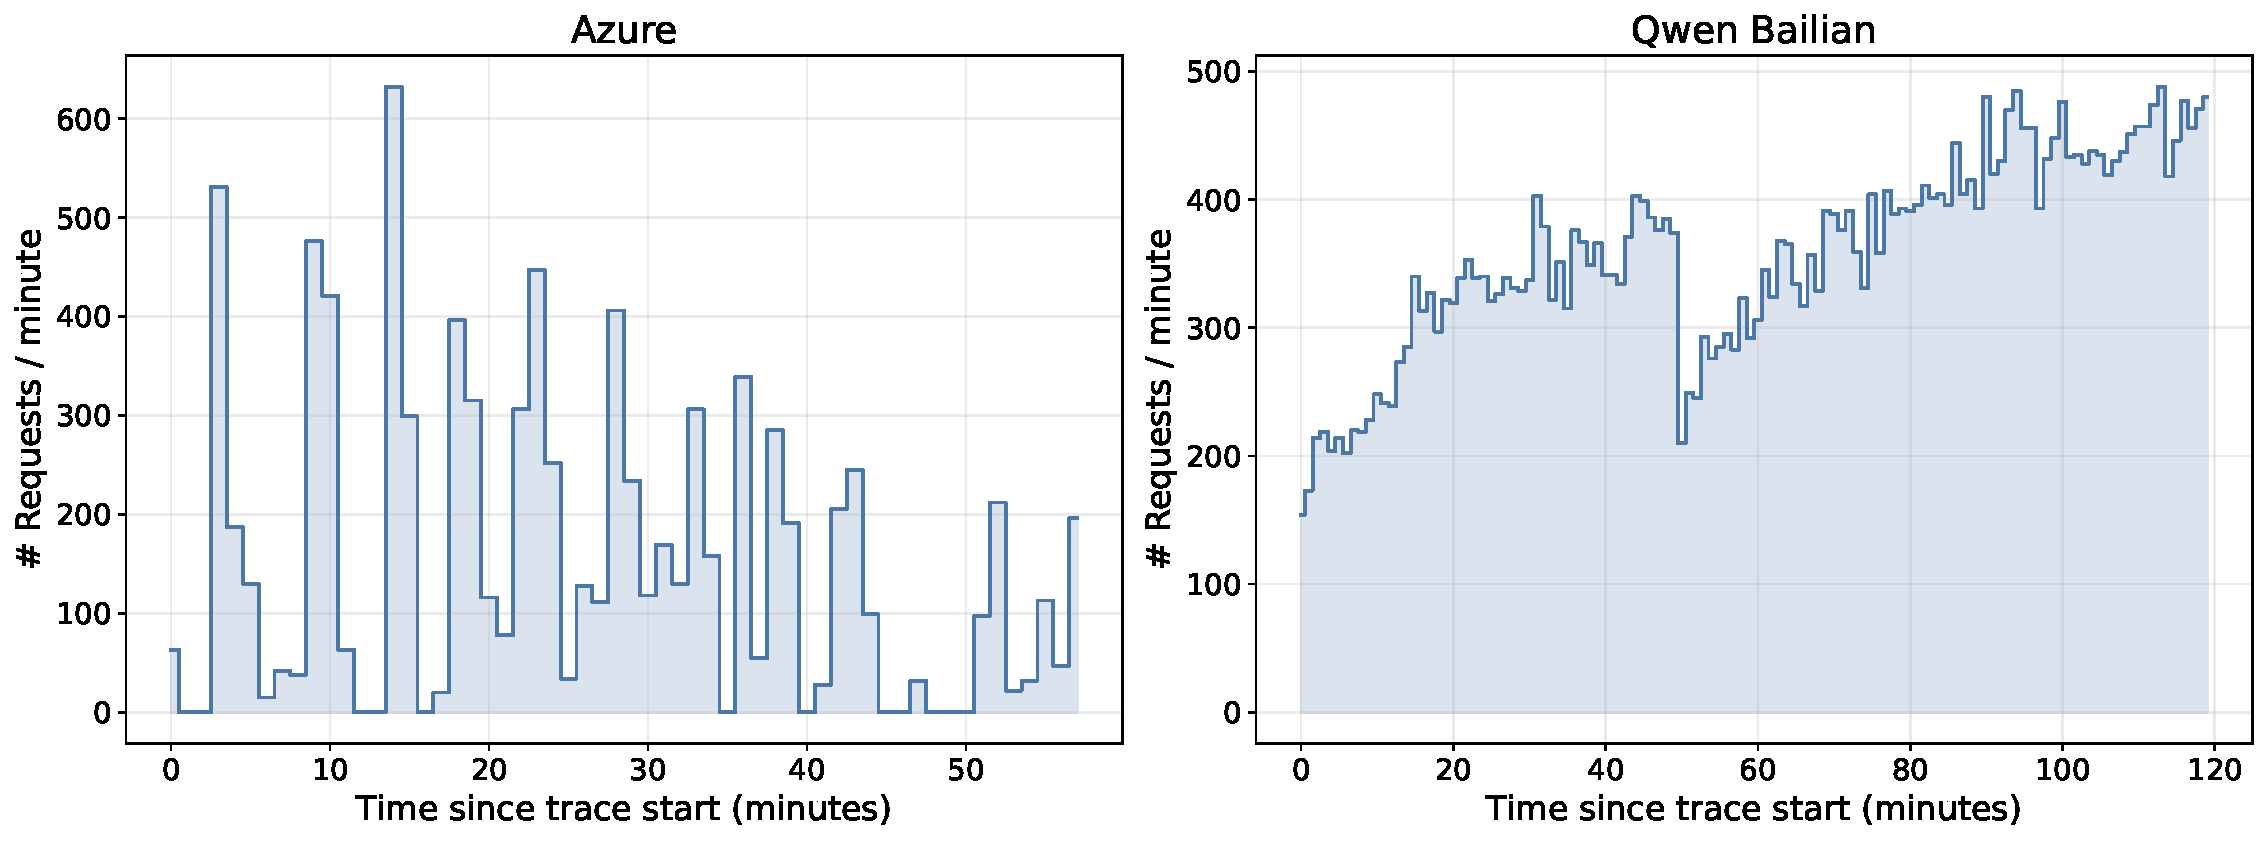
\includegraphics[width=1.0\linewidth]{figures/online-request-trace.pdf}
    \end{center}
    \caption{
        Request arrival patterns of the Azure and Qwen Bailian traces, measured as the number of requests per minute over time.
    }
    \label{fig:online_request_trace}
\end{figure}

We further examine the request-volume dynamics of the two online inference traces used in our end-to-end evaluation, as shown in Figure~\ref{fig:online_request_trace}, and summarize their key statistics in Table~\ref{tab:trace_statistics}.

\textbf{Azure Trace.}
The Azure trace exhibits highly bursty traffic, with frequent alternations between low-load periods and sharp traffic spikes.
Its average arrival rate is 152.05 requests/min, while the peak reaches 632 requests/min, about 4.16$\times$ the average.
Such rapid load fluctuations make SD beneficial during low-load periods, but may cause performance degradation when sudden bursts push the serving system into a high-load regime.
Therefore, this trace is well suited for evaluating whether dynamic SD methods can effectively adapt their SD decisions to rapidly changing serving loads.

\textbf{Qwen Bailian Trace.}
In contrast, the Qwen Bailian trace is considerably smoother and remains under sustained high load for most of its duration.
Its average arrival rate reaches 358.82 requests/min, more than twice the 152.05 requests/min observed in the Azure trace, while its peak is 488 requests/min.
Under such consistently high load, the benefit of SD is limited and can even cause performance degradation, while a large number of requests may accumulate in the waiting queue.
This trace is therefore well suited for evaluating both the Non-SD overhead introduced by dynamic SD mechanisms under high load and the effectiveness of task scheduling strategies in reducing queueing delay.

\begin{table}[H]
    \centering
    \caption{Statistics of the Azure and Qwen Bailian traces.}
    \label{tab:trace_statistics}
    \begin{tabular}{lrrrrr}
        \toprule
        \textbf{Trace} &
        \textbf{\# Requests} &
        \textbf{Duration (min)} &
        \textbf{Avg. Req./min} &
        \textbf{Peak Min.} &
        \textbf{Peak Req.} \\
        \midrule
        Azure         & 8,819  & 57.27  & 152.05 & 14  & 632 \\
        Qwen Bailian  & 43,058 & 119.99 & 358.82 & 113 & 488 \\
        \bottomrule
    \end{tabular}
\end{table}


\clearpage

% 不同硬件平台的资源分析
\section{Serving Capacity Analysis}
\label{resource-analysis}

% 暂时占个位置
\clearpage

% 不同通信频率的影响
\section{Impact of Communication Frequency on System Performance}
\label{communication-frequency}

% 暂时占个位置
\clearpage

% 预测-调度策略的额外开销
\section{Overhead of SpecSys Prediction and Scheduling}
\label{prediction-scheduling-overhead}

% 暂时占个位置
\clearpage

\end{document}
